\chapter{OpenTX: Open Transition System with External State}
\label{ch:ox}

CompCertX, together with its corresponding instance of
the Certified Abstract Language (CAL),
provides a scalable verification framework
successfully applied to verify the
CertiKOS operating system kernel.
The key to the framework's scalability
lies in its capability to decompose the system into
multiple layers
and the interoperability with abstract specifications and states.

While CompCertO provides a solid foundation for compositional verification,
it lacks certain compositional structures needed for complex system verification,
particularly the ability to compose components with heterogeneous interfaces
and manage external state in a modular fashion.
In this chapter, I will enrich CompCertO's composition structures
with additional capabilities to develop a new framework, OpenTX (for Open Transition system with eXternal state).
This framework is shown to
subsume the functionality of CompCertX
while remaining grounded in the open transition system semantics in CompCertO.

As a running example throughout this chapter,
the implementation of the bounded queue
and the ring buffer
in \autoref{fig:bq-code} is used.
The overall objective
is to decompose the correctness proof as follows:
\[
  \begin{prooftree}
    \hypo{L_\kw{bq} \le M_\kw{bq} \odot L_\kw{rb}}
    \hypo{M_\kw{bq} \le \kw{Clight}(\kw{bq.c})}
    \hypo{L_\kw{rb} \le \kw{Clight}(\kw{rb.c})}
    \infer2[monotonicity]{M_\kw{bq} \odot L_\kw{bq} \le \kw{Clight}(\kw{bq.c}) \odot \kw{Clight}(\kw{rb.c})}
    \infer2[transitivity]{L_\kw{bq} \le \kw{Clight}(\kw{bq.c}) \odot \kw{Clight}(\kw{rb.c})}
  \end{prooftree}
\]
With the compiler correctness and linking property,
the end-to-end correctness can be established:
\[
  L_\kw{bq} \le \kw{Asm}(\kw{bq.s} + \kw{rb.s}) \,.
\]
The necessary ingredients of the framework
to enable modular decomposition will be introduced.
In \S\ref{sec:ox:layered} and \S\ref{sec:ox:lifting},
two central operators are presented:
the layered composition operator $\odot$,
which composes individual components
as shown in the proof tree above,
and the state lifting operator $\at$,
which extends the CompCertO semantics
to incorporate external state.
Together,
these operators
transform CompCertO from a certified compiler
into the broader verification framework OpenTX,
thereby recovering the full expressiveness of CompCertX.

To enable fine-grained reasoning about memory state—particularly valuable when
verifying high-level specifications expressed in terms of abstract state
against concrete Clight implementations that manipulate low-level memory data—
\S\ref{sec:ox:separation} examines separation within CompCertO's memory model.
Building on this foundation,
\S\ref{sec:ox:cal} demonstrates how the CAL framework
can be instantiated within the OpenTX framework,
showcasing the practical applicability of the approach.
Finally,
\S\ref{sec:ox:tensor-lens} revisits the stateful construction
in greater detail,
generalizing it to a broader, more flexible form
that extends its applicability to a wider range of verification scenarios.

\begin{table}
  \centering
  \begin{tabular}{ll}
    \toprule
    Notation & Description\\
    \midrule
    $A$, $B$, $C$ & Language Interface \\
    $L: A \twoheadrightarrow B$ & Transition System \\
    $\mathbb{R}: A \twoheadleftrightarrow B $ & Simulation Convention \\
    $\phi: L_1 \le_{\mathbb{R} \twoheadrightarrow \mathbb{S}} L_2$ & Simulation \\
    $L_1 \oplus L_2$ & Linking Operator on Transition Systems (Sec~\ref{bg:compcerto:linking}) \\
    $\mathbb{R} \fatsemi \mathbb{S}$ & Composition of Simulation Conventions \\
    $\mathbb{R} \sqsubseteq \mathbb{S}$ & Refinement on Simulation Conventions \\
    \midrule
    $L_1 \odot L_2$ & Layered Composition of Transition Systems (Sec~\ref{sec:ox:layered}) \\
    $L_1 \otimes L_2$ & Tensor Product of Transition Systems (Sec~\ref{sec:ox:tensor}) \\
    $- \at U$ & Lifting with State $U$ (Sec~\ref{sec:ox:lifting}) \\
    $ \kw{J} \subseteq (\kw{mem} \times \kw{mem}) \times \kw{mem} $ & Join Operation on Memory State (Sec.~\ref{sec:ox:separation}) \\
    $\termi{U}^* : \mathbf{1} \twoheadleftrightarrow U$ & Simulation Convention with Invariance on $U$ (Sec.~\ref{sec:ox:application}) \\
    $[U]$ & Set as Language Interface \\
    $\llbracket U \rrbracket : [U] \twoheadrightarrow [U]$ & Set as Transition System \\
    $f : U \lensarrow V$ & Lens (Sec~\ref{sec:ox:lens}) \\
    $\llbracket f \rrbracket : [U] \twoheadrightarrow [V]$ & Lens as Transition System (Def.~\ref{ox:def:lts-lens}) \\
    $f \circ g$ & Composition of Lenses (Def.~\ref{ox:def:lens-comp}) \\
    \bottomrule
  \end{tabular}
  \caption{Summary of notations}
  \label{tab:ox:notations}
\end{table}

Table~\ref{tab:ox:notations} summarizes the notations used in this chapter.
The upper portion collects those already established in CompCertO,
while the lower portion introduces the new notations specific to this chapter.

\section{Layered Composition}
\label{sec:ox:layered}

Transition systems can be composed
in various ways.
As mentioned in \autoref{sec:bg:compcert-compose},
the linking operator
$\oplus_A : (A \twoheadrightarrow A) \times (A \twoheadrightarrow A)
\rightarrow (A \twoheadrightarrow A)$
enables mutual recursion:
in $L_1 \oplus L_2$,
calls from $L_1$ to $L_2$,
as well as calls from $L_2$ to $L_1$,
are treated as internal calls
and are hidden from the environment.
However,
the composition restricts the two components
to be \emph{homogeneous},
meaning they must share the same language interface
for both outgoing and incoming calls.
In contrast,
a \emph{layered composition} operator $\odot$ is introduced
which is more fundamental and
provides greater flexibility:
\[
  {\odot}_{A,B,C} :
  (B \twoheadrightarrow C) \times
  (A \twoheadrightarrow B) \rightarrow
  (A \twoheadrightarrow C)
  \,.
\]

The transition system
$L_1 \odot L_2$
is depicted in \autoref{fig:ox:ts:comp}.
Incoming calls in $C$ activate $L_1$.
The outgoing calls of $L_1$ in $B$
are handled by $L_2$,
and the outgoing calls of $L_2$
in $A$ are directed to the environment.
The identity transition system $\kw{id}_A$,
as depicted in \autoref{fig:ox:ts:id},
simply passes calls through.

\begin{definition}[Transition system composition]
  The transition system
  $\kw{id}_A : A \twoheadrightarrow A$
  is defined as
  \[
    \kw{id}_A \::=\:
    \big\langle
    A^\que + A^\ans, \:
    \varnothing, \:
    \iota_1, \:
    \iota_1^{-1}, \:
    \iota_2, \:
    \iota_2^{-1}
    \big\rangle
    \,.
  \]
  The composition of
  $
  L_1 = \langle S_1, {\rightarrow_1}, I_1, X_1, Y_1, T_1 \rangle
  : B \twoheadrightarrow C
  $ and $
  L_2 = \langle S_2, {\rightarrow_2}, I_2, X_2, Y_2, T_2 \rangle
  : A \twoheadrightarrow B
  $
  is the transition system
  $
  L_1 \odot L_2 :=
  \langle S, {\rightarrow}, I, X, Y, F \rangle
  : A \twoheadrightarrow C
  $ defined as follows.
  States are taken in the set
  $
  S := S_1 + (S_2 \times S_1)
  $.
  When an incoming question in $C$ activates $L_1$,
  the left summand is used:
  \[
    \begin{prooftree}
      \hypo{q_C \mathrel{I_1} s_1}
      \infer1{q_C \mathrel{I} \iota_1(s_1)}
    \end{prooftree}
    \qquad
    \begin{prooftree}
      \hypo{s_1 \rightarrow_1 s_1'}
      \infer1{\iota_1(s_1) \rightarrow \iota_1(s_1')}
    \end{prooftree}
    \qquad
    \begin{prooftree}
      \hypo{s_1 \mathrel{F_1} r_C}
      \infer1{\iota_1(s_1) \mathrel{F} r_C}
    \end{prooftree}
  \]
  When $L_1$ makes an outgoing question in $B$,
  its current state is saved and
  the question activates $L_2$.
  The execution then
  operates on the state of $L_2$
  until a final state of $L_2$ is reached
  and $L_1$ is resumed:
  \begin{align*}
    \begin{prooftree}
      \hypo{s_1 \mathrel{X_1} q_B}
      \hypo{q_B \mathrel{I_2} s_2}
      \infer2{\iota_1(s_1) \rightarrow \iota_2(s_2, s_1)}
    \end{prooftree}
    \quad
    \begin{prooftree}
      \hypo{s_2 \rightarrow_2 s_2'}
      \infer1{\iota_2(s_2, s_1) \rightarrow \iota_2(s_2', s_1)}
    \end{prooftree}
    \quad
    \begin{prooftree}
      \hypo{s_2 \mathrel{X_2} q_A}
      \infer1{\iota_2(s_2, s_1) \mathrel{X} q_A}
    \end{prooftree}
  \end{align*}
  \vspace{-3em}
  \begin{align*}
    \begin{prooftree}
      \hypo{r_A \mathrel{Y_2^{s_2}} s_2'}
      \infer1{r_A \mathrel{Y^{\iota_2(s_2, s_1)}} \iota_2(s_2', s_1)}
    \end{prooftree}
    \quad
    \begin{prooftree}
      \hypo{s_2 \mathrel{F_2} r_B}
      \hypo{r_B \mathrel{Y_1^{s_1}} s_1'}
      \infer2{\iota_2(s_2, s_1) \rightarrow \iota_1(s_1')}
    \end{prooftree}
  \end{align*}

\end{definition}

\begin{figure}
  \begin{subfigure}{0.45\textwidth}
    \centering
    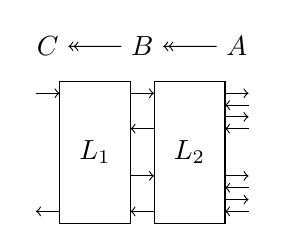
\begin{tikzpicture}[yscale=0.15,xscale=0.30]
      \draw (1,-1) rectangle (4,11) node[midway] {$L_1$};
      \draw (5,-1) rectangle (8,11) node[midway] {$L_2$};
      %\draw (5,-1) rectangle (8,4) node[midway] {$L_2$};
      \draw[->] (0,10) -- (1,10) node[above=1em,midway] (C) {$C$};
      \draw[->] (4,10) -- (5,10) node[above=1em,midway] (B) {$B$};
      \draw[->] (8,10) -- (9,10) node[above=1em,midway] (A) {$A$};
      \draw[->] (9,9) -- (8,9);
      \draw[->] (8,8) -- (9,8);
      \draw[->] (9,7) -- (8,7);
      \draw[->] (5,7) -- (4,7);
      \draw[->] (4,3) -- (5,3);
      \draw[->] (8,3) -- (9,3);
      \draw[->] (9,2) -- (8,2);
      \draw[->] (8,1) -- (9,1);
      \draw[->] (9,0) -- (8,0);
      \draw[->] (5,0) -- (4,0);
      \draw[->] (1,0) -- (0,0);
      \draw[->>] (A) -- (B);
      \draw[->>] (B) -- (C);
    \end{tikzpicture}
    \subcaption{Composition}
    \label{fig:ox:ts:comp}
  \end{subfigure}
  \begin{subfigure}{0.45\textwidth}
    \centering
    \begin{tikzpicture}[yscale=0.15,xscale=0.30]
      \draw (5,-1) rectangle (8,4) node[midway] {$\kw{id}_A$};
      \draw[->] (4,3) node[left] {\scriptsize $q \in A^\que$}
      -- (5,3) node[above=2em,midway] (A2) {$A$};
      \draw[->] (8,3) -- (9,3) node[above=2em,midway] (A1) {$A$}
      node[right] {\scriptsize $q$};
      \draw[->] (9,0) node[right] {\scriptsize $r \in A^\ans$} -- (8,0);
      \draw[->] (5,0) -- (4,0) node[left] {\scriptsize $r$};
      \draw[->>] (A1) -- (A2);
    \end{tikzpicture}
    \vspace{1ex}
    \subcaption{Identity}
    \label{fig:ox:ts:id}
  \end{subfigure}
  \caption{Informal description of CompCertO's
    transition system
  under \emph{layered} composition}
  \label{fig:ox:ts}
\end{figure}
In a layered composition $L_1 \odot L_2$,
$L_1$ is referred to as the \textit{client},
and $L_2$ as the \textit{handler}.

\subsection{Normalization}

The identity LTS and the layered composition are expected to form a categorical
structure. However, when composing with the identity LTS to the left of an LTS
$L$, the composite LTS $\kw{id} \odot L$ initiates at state
$\iota_1(\iota_1(q))$ upon an incoming question $q$. This step is impossible to
be simulated by the original LTS $L$, whose initial step must choose a state.
Similarly, at final state, the LTS $L$ chooses an answer $r$ from its final
state. However, the composite LTS $\kw{id} \odot L$ must have already known the
answer so that it can move from the state $\iota_1(\iota_2(r))$ to the answer
$r$. Symmetrically, the same problem happens when the right identity law and the
other side of questions and answers are considered.

Conventionally, the standard solution to step mismatch is to allow for
``stuttering steps''. However, the CompCertO's simulation only allows for such
stuttering steps for the internal transition steps, and the transitions at the
outgoing and incoming boundaries must be lock-step. Instead of relaxing
CompCertO's simulation, it is observed that composing with the identity LTS
internalizes the transitions on the LTS boundary. As a consequence, the
following simulations can be established:
\[
  \kw{id} \odot \kw{id} \odot L = \kw{id} \odot L
  \qquad
  L \odot \kw{id} \odot \kw{id} = L \odot \kw{id}
\]
Thus, normalized LTS is defined as follows:
\[
  \kw{norm}(L) \::=\: \kw{id} \odot L \odot \kw{id}
\]
This normalization ensures that
both the associativity and the identity law are satisfied.
For the remainder of this thesis,
attention is restricted to normalized LTSs
and therefore the notation $\kw{norm}(L)$ is omitted
for brevity.

\begin{theorem}
  \label{thm:ox:ts}
  The open transition system in CompCertO forms a category $\mathbf{TS}$.
\end{theorem}

\subsection{Linking}

Another important property of the layered composition is that layered
composition of Asm programs be implemented by syntactic linking of the programs,
which plays an important role in the end-to-end verification framework. This
property is enabled by the under-approximation of the CompCertO's original
notion of horizontal composition.
\[
  \kw{Asm}(p_1) \odot \kw{Asm}(p_2)
  \le \kw{Asm}(p_1) \oplus \kw{Asm}(p_2)
  \le \kw{Asm}(p_1 + p_2)
\]

\subsubsection{Footprint}

CompCertO associates each translation system $L: A \twoheadrightarrow B$ with a
predicate $V_L \subseteq B^\que$ for identifying the questions that are accepted
by the translation system $L$. More concretely, in the composite transition
system $L_1 \oplus L_2$, when $L_1$ is at the position to make an external call
$q$, either of the following situations occurs:
\begin{itemize}
  \item $q$ escapes as an outgoing question of $L_1 \oplus L_2$ if $q \notin V_{L_2}$
  \item $q$ initiates $L_2$ as an incoming question if $q \in V_{L_2}$
\end{itemize}
The situation is symmetric for $L_2$. A subtlety with the validity check is that
it is used both covariantly and contravariantly. So the simulation between two
transition systems implies they have the same validity predicate.

For horizontal composition, the validity predicate is the union of the two
transition systems:
\[
  V_{L_1 \oplus L_2} := V_{L_1} \cup V_{L_2}
\]
Therefore, to prove the under-approximation, it must be defined:
\[
  V_{L_1 \odot L_2} := V_{L_1} \cup V_{L_2}
\]
However, in general, $L_1$ and $L_2$ may not use the same language interface so
the valid question sets cannot be simply unioned. Therefore the
valid question set is generalized to be the language-agnostic footprint set $P_L \subseteq
\mathcal{P}(\kw{ident})$, which contains the identifiers associated with the
valid questions.

The identity transition system has an empty footprint set but it accepts all
questions.

\subsubsection{Under-approximation}

The horizontal composition uses valid question sets for the following situations:
\begin{itemize}
  \item when an incoming question $q$ arrives, the component whose footprint
    includes $q$ is activated. It gets stuck if neither component accepts the
    question $q$.
  \item when either component makes an external call $q$, it can only escape as
    an outgoing question if $q$ falls outside both components' footprint.
    Otherwise, the corresponding component is activated.
\end{itemize}

Thus, to prove the under-approximation, it must be shown that the layered composition
obeys the behavior of the horizontal composition or gets stuck. Particularly, it is necessary to show:
\begin{itemize}
  \item if the incoming question $q$ activates $L_1$, it must be in the
    footprint of $L_1$
  \item if the outgoing question $q$ escapes, it must be outside both components'
    footprint
\end{itemize}

The first condition seems trivial but an obvious counterexample exists%
---the identity transition system. To solve this problem, the scope is limited to
transition systems that are associated with concrete programs. For concrete
programs, they have the following properties:
\begin{itemize}
  \item incoming questions are always in the footprint
  \item outgoing questions are always outside the footprint
\end{itemize}
Additionally, it is required that outgoing questions of $L_2$ are outside the footprint of
$L_1$ to complete the proof.

\begin{remark}
  Another possible route to prove the under-approximation with side conditions is
  to use the footprint to guide the behavior of layered composition. For example,
  it could be required that for $L_1 \odot L_2$, when $L_2$ makes an external call
  $q$, $q \notin V_{L_1}$. However, such conditions complicate the proof of
  associativity of the layered composition. Consider one of the simulation laws:
  \[
    L_1 \odot (L_2 \odot L_3) \le (L_1 \odot L_2) \odot L_3
  \]
  When $L_2$ is at the position to make an external call $q$ to $L_3$, the target
  transition system must prove $q$ cannot be accepted by $L_1$ so that it can
  escape the composite transition system $L_1 \odot L_2$ as an outgoing question.
  But this information is never provided by the source transition system.
\end{remark}

\subsection{Properties of Layered Composition}

The key result is that simulation squares are closed
under horizontal composition,
corresponding to the layered composition operator $\odot$
used for combining components side by side.

\begin{theorem}[Horizontal composition of simulation squares]
  The simulation squares compose along the layered composition:
  \[
    \begin{prooftree}
      \hypo{\phi: L_1 \le_{\mathbb{S} \twoheadrightarrow \mathbb{T}} L'_1}
      \hypo{\psi: L_2 \le_{\mathbb{R} \twoheadrightarrow \mathbb{S}} L'_2}
      \infer2[\kw{sim}-$\odot$]{\phi \odot \psi: L_1 \odot L_2 \le_{\mathbb{R} \twoheadrightarrow \mathbb{T}} L'_1 \odot L'_2}
    \end{prooftree}
    \qquad
    \begin{array}{c}
      \begin{tikzcd}[row sep=2ex, column sep=2ex]
        A_1 \ar[rr, twoheadrightarrow, "L_2"]
        \ar[dd, leftrightarrow, "\mathbb{R}"]
        && B_1 \ar[rr, twoheadrightarrow, "L_1"]
        \ar[dd, leftrightarrow, "\mathbb{S}"]
        && C_1
        \ar[dd, leftrightarrow, "\mathbb{T}"]
        \\
        & \psi && \phi
        \\
        A_2 \ar[rr, twoheadrightarrow, "L'_2"] && B_2 \ar[rr, twoheadrightarrow, "L'_1"] && C_2
      \end{tikzcd}
    \end{array}
  \]
\end{theorem}

The rule $\kw{sim}$-$\odot$
composes simulation squares horizontally,
and is therefore also referred to as the horizontal composition.
It complements the rule $\kw{sim}$-$\fatsemi$,
which composes simulation squares vertically.
Together,
these two composition rules
form the core expressive power of the framework.
Overall,
the compositional structure of the model
can be summarized in the following way.
\begin{theorem}
  \label{thm:ox:tsc}
  Language interfaces,
  open transition systems,
  simulation conventions,
  and simulation properties
  form a thin double category $\mathbf{TSC}$.
\end{theorem}

This characterization
gives a formal underpinning
to the notions of horizontal and vertical composition.

\subsection{Properties of Identity Transition System}

The identity transition system $\kw{id}$
provides a way to
restate the refinement order
between simulation conventions
in terms of a simulation square.
\begin{theorem}
  \label{thm:ox:sc-ref}
  Consider simulation conventions
  $\mathbb{R}, \mathbb{S} : A \twoheadleftrightarrow B$,
  the following property holds:
  \[
    \begin{prooftree}
      \hypo{\mathbb{S} \sqsubseteq \mathbb{R}}
      \infer1{\kw{id}_A \le_{\mathbb{R} \twoheadrightarrow \mathbb{S}} \kw{id}_B}
    \end{prooftree}
    \qquad \qquad \qquad
    \begin{tikzcd}[row sep=2ex, column sep=2ex]
      A \ar[rr, "\kw{id}_A"] \ar[dd, leftrightarrow, "\mathbb{R}"'] && A \ar[dd, leftrightarrow, "\mathbb{S}"] \\
      &\mathbb{S} \sqsubseteq \mathbb{R} & \\
      B \ar[rr, "\kw{id}_B"] && B
    \end{tikzcd}
  \]
\end{theorem}
For convenience, the notation
$\phi^r(\mathbb{R}) : \kw{id}_A \le_{\mathbb{R} \twoheadrightarrow \mathbb{R}} \kw{id}_B$
is used for the simulation square derived from the refinement convention $\mathbb{R}$.
Similarly,
the notation $\phi^l(L) : L \le L$
is used to denote the simulation square derived from the transition system $L$
with the identity simulation convention.
This dual perspective is depicted in the diagrams that follow.
\[
  \begin{tikzcd}[row sep=2ex, column sep=2ex]
    A \ar[rr, "\kw{id}_A"] \ar[dd, leftrightarrow, "\mathbb{R}"'] && A \ar[dd, leftrightarrow, "\mathbb{R}"] \\
    &\phi^r(\mathbb{R}) & \\
    B \ar[rr, "\kw{id}_B"] && B
  \end{tikzcd}
  \qquad
  \qquad
  \begin{tikzcd}[row sep=2ex, column sep=2ex]
    A \ar[rr, "L"] \ar[dd, leftrightarrow, "\kw{id}"'] && B \ar[dd, leftrightarrow, "\kw{id}"] \\
    &\phi^l(L) & \\
    A \ar[rr, "L"] && B
  \end{tikzcd}
\]

The theory of double categories also offers
an additional layer of structure: companions and conjoints.
These provide a systematic way of
relating horizontal and vertical morphisms.
In this setting, this means that certain transition systems
can also be viewed as simulation conventions.

\begin{definition}
  \label{def:ox:companion}

  A transition system $L : A \twoheadrightarrow B$ is said to have
  \begin{itemize}
    \item a companion $L^* : A \twoheadleftrightarrow B$ when
      $\phi_1^{cp}(L) : \kw{id}_A \le_{\kw{id} \twoheadrightarrow L^*} L$
      and
      $\phi_2^{cp}(L) : L \le_{L^* \twoheadrightarrow \kw{id}} \kw{id}_B$
    \item a conjoint $L_* : B \twoheadleftrightarrow A$ when
      $\phi_1^{cj}(L) : \kw{id}_B \le_{L_* \twoheadrightarrow \kw{id}} L$
      and
      $\phi_2^{cj}(L) : L \le_{\kw{id} \twoheadrightarrow L_*} \kw{id}_A$
  \end{itemize}

  The simulation squares have the following shape:
  \begin{center}
    \hspace{-2.5em}
    \begin{tikzcd}[row sep=2ex, column sep=2ex]
      A \ar[rr, "\kw{id}_A"] \ar[dd, leftrightarrow, "\kw{id}"'] && A \ar[dd, leftrightarrow, "L^*"] \\
      &\phi_1^{cp}(L) & \\
      A \ar[rr, "L"] && B
    \end{tikzcd}
    \quad
    \begin{tikzcd}[row sep=2ex, column sep=2ex]
      A \ar[rr, "L"] \ar[dd, leftrightarrow, "L^*"'] && B \ar[dd, leftrightarrow, "\kw{id}"] \\
      &\phi_2^{cp}(L) & \\
      B \ar[rr, "\kw{id}_B"] && B
    \end{tikzcd}
    \quad
    \begin{tikzcd}[row sep=2ex, column sep=2ex]
      B \ar[rr, "\kw{id}_B"] \ar[dd, leftrightarrow, "L_*"'] && B \ar[dd, leftrightarrow, "\kw{id}"] \\
      &\phi_1^{cj}(L) & \\
      A \ar[rr, "L"] && B
    \end{tikzcd}
    \quad
    \begin{tikzcd}[row sep=2ex, column sep=2ex]
      A \ar[rr, "L"] \ar[dd, leftrightarrow, "\kw{id}"'] && B \ar[dd, leftrightarrow, "L_*"] \\
      &\phi_2^{cj}(L) & \\
      A \ar[rr, "\kw{id}_A"] && A
    \end{tikzcd}
  \end{center}

\end{definition}

These properties mean that
although the transition systems and simulation conventions
are fairly different in nature,
sometimes a component can be treated as both.
In particular,
for certain simulation statements,
it can be chosen whether a
component should appear as a transition system
or as a simulation convention.
This generally affords additional flexibility
in the decomposition of proofs.

Companions and conjoints satisfy standard adjunction properties,
mirroring their categorical counterparts.
These properties are especially useful for
``cancelling'' intermediate components
when composing simulations.
\begin{theorem}
  \label{thm:ox:cp-cj-adj}
  By simple diagram chasing,
  the following adjunction properties are obtained:
  \[
    \kw{id} \sqsubseteq L_* \fatsemi L^*
    \qquad
    L^* \fatsemi L_* \sqsubseteq \kw{id}
  \]
\end{theorem}

Concrete examples of transition systems
with companions and conjoints
will be given in \autoref{sec:ox:lens}.
Practical uses of these constructs will also be encountered in
\autoref{sec:oe:sim-encap}
and
\autoref{sec:oe:clightp-correctness}.

\section{Lifting with State}
\label{sec:ox:lifting}

In this section,
the state lifting that equips the CompCertO semantics
with external states is introduced.

\subsection{Layer Interface}

The language interfaces
of CompCertO languages
are attached with the memory state
alongside with the questions and answers,
expressed as $\C \at \kw{mem}$ for example.
This can be generalized
to an arbitrary language interface $A$
with a set of states $U$.
The corresponding state-carrying layer interface
$A \mathbin@ U$
is defined as:
\[
  A \mathbin@ U := \langle A^\que \times U, A^\ans \times U \rangle
\]
A transition system $L: A \mathbin@ U \twoheadrightarrow B \mathbin@ V$ handles
the state of type $V$ that is passed from the environment, and uses the state of
type $U$ to interact with its downstream components.

The construction admits the following structural isomorphisms, and obvious
isomorphic transformations on language interfaces will be implicitly inserted in
the rest of this thesis.
\[
  \C \mathbin@ S \mathbin@ T \cong \C \mathbin@ (S \times T) \cong \C \mathbin@ (T \times S)
  \qquad
  \C \mathbin@ \{*\} \cong \C
  \qquad
  \C \mathbin@ \varnothing \cong \mathbf{0}
\]

Other than using the memory as the state,
abstract state can be used
and transition systems can be defined
to execute on the abstract state,
which serve as specifications for the program in Fig.~\ref{fig:bq-code}.
In particular,
the specification $L_\kw{bq}$
gives an abstract description of the code
by representing the queue state as a sequence $\vec{q}$.
\[
  \begin{aligned}
    & L_\kw{bq} : \mathbf{0} \twoheadrightarrow \C \mathbin@ D_\kw{bq} \\
    & D_\kw{bq} := V^*
  \end{aligned}
  \qquad
  \begin{aligned}
    L_\kw{bq} & \vDash \kw{enq}(v)@\vec{q} \rightarrowtail *@\vec{q}v \\
    L_\kw{bq} & \vDash \kw{deq}()@\vec{q}v \rightarrowtail v@\vec{q}
  \end{aligned}
  \qquad\text{where}\qquad
  \vec{q} \in D_\kw{bq},
  v \in V
\]
The empty language interface $\mathbf{0} := \langle \varnothing, \varnothing
\rangle$ indicates that the specifications $L_\kw{bq}$ does not make any
outgoing questions.
Likewise $L_\kw{rb}$ uses the data $(b, c_1, c_2)$
to represent the contents of the buffer and the counter values.
The behavior of the ring buffer
translates to the following transition system,
which captures the behavior of the $\kw{rb.c}$.
\[
  \begin{aligned}
    L_\kw{rb}& : \mathbf{0} \twoheadrightarrow \C \mathbin@ D_\kw{rb}\\
    D_\kw{rb}& := V^N \times \mathbb{N} \times \mathbb{N}
  \end{aligned}
  \qquad
  \begin{aligned}
    L_\kw{rb} & \vDash \kw{set}(i, v)@b, c_1, c_2
    \rightarrowtail *@(b[i \mapsto v], c_1, c_2) \\
    L_\kw{rb} & \vDash \kw{get}(i)@b, c_1, c_2
    \rightarrowtail b[i]@(b, c_1, c_2)\\
    L_\kw{rb} & \vDash \kw{inc_1}()@b, c_1, c_2
    \rightarrowtail *@(b, (c_1 + 1) \% N, c_2) \\
    L_\kw{rb} & \vDash \kw{inc_2}()@b, c_1, c_2
    \rightarrowtail *@(b, c_1, (c_2 + 1) \% N)
  \end{aligned}
\]
Finally,
$\kw{bq.c}$ does not use any state of its own
and can be described by the following specification.
\[
  M_\kw{bq} : \C \twoheadrightarrow \C
  \qquad
  \begin{aligned}
    M_\kw{bq} & \vDash \kw{enq}(v) \sysstep
    (\kw{inc_2}() \envstep i) \sysstep
    (\kw{set}(i, v) \envstep *) \sysstep
    * \\
    M_\kw{bq} & \vDash \kw{deq}() \sysstep
    (\kw{inc_1}() \envstep i) \sysstep
    (\kw{get}(i) \envstep v) \sysstep
    v
  \end{aligned}
\]
With these specifications,
a correctness proof is hoped to be decomposed
along the following lines:
\[
  \phi_\kw{spec} : L_\kw{bq}
  \le_{\mathbf{0} \twoheadrightarrow ?}
  M_\kw{bq} \! \mathbin{\text{``}{\odot}\text{''}} L_\kw{rb}
  \quad\:
  \phi_\kw{bq} : M_\kw{bq}
  \le_{? \twoheadrightarrow ?}
  \kw{Clight}(\kw{bq.c})
  \quad\:
  \phi_\kw{rb} : L_\kw{rb}
  \le_{\varnothing \twoheadrightarrow ?}
  \kw{Clight}(\kw{rb.c})
\]
However, the different types of states
prevent the components
from being composed directly.
To make the approach outlined above practical,
$@$ must be turned into a proper composition principle
and its action must be established on
transition systems,
simulation conventions and
simulation squares.

\subsection{Transition System with External State}
\label{sec:ox:lifting-lts}

The construction ${-} \at U$ is outlined
as it acts on transition systems
in the case of a fixed set $U$.
Namely,
given $L : A \twoheadrightarrow B$,
the transition system
$
L \at U : A \at U \twoheadrightarrow B \at U
$
transparently passes along
a state component of type $U$ as follows:
\begin{equation} \label{eqn:slift}
  \begin{prooftree}
    \hypo{
      L \:\vDash\: q \rightarrowtail
      (m_1 \leadsto n_1) \rightarrowtail
      \cdots \rightarrowtail
      (m_n \leadsto n_n) \rightarrowtail
      r
    }
    \infer1{
      L \at U \:\vDash\: q\at u_0 \rightarrowtail
      (m_1\at u_0 \leadsto n_1\at u_1) \rightarrowtail
      \cdots \rightarrowtail
      (m_n\at u_{n-1} \leadsto n_n\at u_n) \rightarrowtail
      r\at u_n
    }
  \end{prooftree}
\end{equation}
Here, the value $u_0 \in U$
is initially received from the environment as part of the incoming question.
$L \mathbin@ U$ then mirrors the execution of $L$
but keeps track of this additional state component.
The state is attached to any outgoing question in $A$
and updated when the corresponding answer is received.
When $L$ terminates,
the final value of the state is returned with the answer in $B$.

\begin{definition}[Lifting Transition System]
  Given a transition system
  $L: A \twoheadrightarrow B = \langle S, \rightarrow, I, X, Y, F \rangle$,
  the lifting transition system $L \at U : A \at U \twoheadrightarrow B \at U$
  is defined as
  \[
    L \at U \::=\: \langle S \times U, \rightarrow, I \times =_U, X \times =_U, Y_U, F \times =_U \rangle
    \qquad
    \begin{prooftree}
      \hypo{n \mathbin{Y^s} s'}
      \infer1{(n, u') \mathbin{Y^{(s, u)}_U} (s', u')}
    \end{prooftree}
  \]
\end{definition}

In the previous section,
the correctness property $\phi_\kw{bq}$ was unable to be stated
due to the difference in type.
The requirement can now be formulated
$
\phi_\kw{bq} : M_\kw{bq} \at \kw{mem} \le \kw{Clight}(\kw{bq.c})
$,
which expresses that $\kw{bq.c}$
makes the outgoing calls prescribed by $M_\kw{bq}$
but does not modify the global memory state.

Further,
$\at$ can be used to interface
$M_\kw{bq} : \C \twoheadrightarrow \C$ with the specification
$L_\kw{rb} : \mathbf{0} \twoheadrightarrow \C \at D_\kw{rb}$.
The result
$
(M_\kw{bq} \at D_\kw{rb}) \odot L_\kw{rb} :
\mathbf{0} \twoheadrightarrow \C \at D_\kw{rb}
$
uses the construction
$M_\kw{bq} \at D_\kw{rb} :
\C \at D_\kw{rb}
\twoheadrightarrow
\C \at D_\kw{rb}$
which allows $M_\kw{bq}$ to
``pass through'' the abstract data $D_\kw{rb}$
on which $L_\kw{rb}$ operates.

\subsection{Simulation Convention}

The $\at$ construction can be further extended
to act on simulation conventions.
A relation-carrying simulation convention
$\mathbb{R} \at R : A \at U \twoheadleftrightarrow B \at V$
for a simulation convention $\mathbb{R}: A \twoheadleftrightarrow B$
and a relation $R \subseteq U \times V$
simply uses the relation $R$
to relate the additional state on questions and answers:
\[
  (\mathbb{R}\at R)^\que := \mathbb{R}^\que \times R \qquad
  (\mathbb{R}\at R)^\ans := \mathbb{R}^\ans \times R
\]
Similar to the way that
the state is passed through
the execution of the transition system,
a relation between the states can be passed through the
steps of the simulation.
\[
  \begin{prooftree}
    \hypo{\phi: L_1 \le_{\mathbb{R} \twoheadrightarrow \mathbb{S}} L_2}
    \infer1{\phi \at R: L_1 \at U
      \le_{\mathbb{R} \at R \twoheadrightarrow \mathbb{S} \at R}
    L_2 \at V}
  \end{prooftree}
\]

% \subsubsection{Lifting}

% \[
%   \begin{prooftree}
%     \hypo{\phi: L_1 \le_{R_1 \twoheadrightarrow R_2} L_2}
%     \hypo{\kw{id}_S: \kw{id}_U \le_{S \twoheadrightarrow S} \kw{id}_V}
%     \infer2{\phi \mathbin@ \kw{id}_S: L_1 \mathbin@ U
%       \le_{R_1 \times S \twoheadrightarrow R_2 \times S}
%     L_2 \mathbin@ V}
%   \end{prooftree}
% \]
% \todo{add a figure to summarize lifting state, lifting relation, lifting sc}
% Note that here $S: U \Leftrightarrow V$ is a simulation convention instead of a
% relation between $U$ and $V$, so we use the product operator $\times : A_1
% \Leftrightarrow B_1 \times A_2 \Leftrightarrow B_2 \rightarrow A_1 \times A_2
% \Leftrightarrow B_1 \times B_2$ on $R_1$ and $S$ instead of the lifting operator
% $@$. In particular, we can define the following simulation convention $\termi{D}
% ^*: 1 \Leftrightarrow D$:
% \[
%   \termi{D}^* := \langle D, \termi{D}^\que, \termi{D}^\ans \rangle \qquad
%   d \:\vDash\: * \mathrel{\termi{D}^\que} d \qquad
%   d \:\vDash\: * \mathrel{\termi{D}^\ans} d
% \]
% This simulation convention conveys the idea that the data $d$ in the answer must
% be kept unchanged as in the question.

% Functoriality of $@$.
% \[
%   (L_1 \odot L_2) \mathbin@ S \equiv (L_1 \mathbin@ S) \odot (L_2 \mathbin@ S)
% \]

\subsection{A Walkthrough of the Example}

With the state lifting operator $\at$
and
the layered composition $\odot$,
the verification of the example
in Fig.~\ref{fig:bq-code} can be completed

\subsubsection{Verifying Ring Buffer}
\label{sec:ox:rb1}

For the first step,
the correctness of the program $\kw{rb.c}$
with respect to the specification $L_\kw{rb}$ is considered.
The specification $L_\kw{rb}$ operates
on the abstract state $D_\kw{rb}$
and the program $\kw{Clight}(\kw{rb.c})$
operates on the memory $\kw{mem}$.
So the following relation $R_\kw{rb}$
is defined to relate the abstract state $D_\kw{rb}$ and the memory $\kw{mem}$:
\begin{align*}
  (buf, c_1, c_2) \mathrel{R_\kw{rb}} m \ :\Leftrightarrow\
  & \kw{se}(\kw{c_1}) = b_1 \:\wedge\: m[b_1, 0] = \kw{Vint}(c_1) \\
  \ \wedge\  & \kw{se}(\kw{c_2}) = b_2 \:\wedge\: m[b_2, 0] = \kw{Vint}(c_2) \\
  \ \wedge\  & \kw{se}(\kw{buf}) = b_{buf}
  \ \wedge\ \forall i \in [0, N). m[b_{buf}, i * 4] = \kw{Vint}(buf[i])
\end{align*}
where $\kw{se}$ is the symbol table
that maps the variable names to their corresponding
blocks in the memory.

Then the following simulation is proved:
\[
  \phi_\kw{rb} \::\: L_\kw{rb}
  \:\le_{\mathbf{0} \twoheadrightarrow \kw{id}_\mathcal{C} \mathbin@ R_\kw{rb}}\:
  \kw{Clight}(\kw{rb.c})
\]
It is worth mentioning that the memory may contain other blocks in addition to
those corresponding to the abstract state $D_\kw{rb}$. They are irrelevant to
the proof itself but for the purpose of composition the guarantee that other
blocks are not changed is necessary. This problem will be solved in later
sections.

\subsubsection{Verifying Bounded Queue}

The correctness of the bounded queue program $\phi_\kw{bq}$
has been shown in \S\ref{sec:ox:lifting-lts}.
Unlike the ring buffer specification
and program which operates on states at
different abstraction level,
the bounded queue does not introduce any state.
So in $\phi_\kw{bq}$ the specification $M_\kw{bq}$
is lifted with the memory to
reflect the fact that the program $\kw{bq.c}$
does not modify the memory state.
However, the simulation $\phi_\kw{bq}$
cannot be directly composed with the
simulation $\phi_\kw{rb}$
because of the mismatch of the language interfaces.
To remedy this,
the specification $M_\kw{bq}$ must instead be lifted
with the state $D_\kw{rb}$
and the relation $R_\kw{rb}$ between $D_\kw{rb}$
and the memory must be maintained throughout the simulation:
\[
  \phi'_\kw{bq} \::\: M_\kw{bq} \mathbin@ D_\kw{rb}
  \:\le_{\kw{id}_\C\mathbin@ R_\kw{rb}
    \twoheadrightarrow
  \kw{id}_\C \mathbin@ R_\kw{rb}}\:
  \kw{Clight}(\kw{bq.c})
\]

\subsubsection{Putting Together}
\label{sec:ox:putting-together}

From the view of data abstraction, the above two steps have managed to bridge
the abstraction gap between CompCertO's memory and the low-level state
$D_\kw{rb}$. The last step is to fill in the gap between the specifications
operate on the high-level state $D_\kw{bq}$ and the low-level state $D_\kw{rb}$:
\[
  \phi_\kw{spec} \::\: L_\kw{bq} \:\le_{\mathbf{0} \twoheadrightarrow \kw{id}_\C \at R_\kw{bq}}\:
  (M_\kw{bq} \at D_\kw{rb}) \ \odot \ L_\kw{rb}
\]
where $R_\kw{bq} \subseteq D_\kw{bq} \times D_\kw{rb}$ relates the
abstract state of the bounded queue and the ring buffer. With all the
ingredients, the complete proof can be established:
\[
  \phi_\kw{spec} \:\fatsemi\: (\phi'_\kw{bq} \odot \phi_\kw{rb}) \::\:
  L_\kw{bq} \:\le_{\mathbf{0} \twoheadrightarrow
  \kw{id}_\C \at R_\kw{bq} \:\fatsemi\: \kw{id}_\C \at R_\kw{rb}}\:
  \kw{Clight}(\kw{bq.c}) \odot \kw{Clight}(\kw{rb.c})
\]
The following diagram illustrates the proof:
\[
  \begin{tikzcd}[row sep=0.5cm, column sep=0.5cm]
    \mathbf{0}
    \ar[rrrr, "L_\kw{bq}"]
    \ar[dd, leftrightarrow, "\mathbf{0}"']
    &&&& \C \at D_\kw{bq}
    \ar[dd, leftrightarrow, "\kw{id}_\C \at R_\kw{bq}"]
    \\
    && \phi_\kw{spec} && \\
    \mathbf{0}
    \ar[rr, "L_\kw{rb}"]
    \ar[dd, leftrightarrow, "\mathbf{0}"']
    && \C \at D_\kw{rb}
    \ar[rr, "M_\kw{bq} \at D_\kw{rb}"]
    \ar[dd, leftrightarrow, "\kw{id}_\C \at R_\kw{rb}"']
    && \C \at D_\kw{rb}
    \ar[dd, leftrightarrow, "\kw{id}_\C \at R_\kw{rb}"]
    \\
    & \phi_\kw{rb} && \phi'_\kw{bq} & \\
    \C \at \kw{mem}
    \ar[rr, "\kw{Clight}(\kw{bq.c})"]
    && \C \at \kw{mem}
    \ar[rr, "\kw{Clight}(\kw{rb.c})"]
    && \C \at \kw{mem} \\
  \end{tikzcd}
\]

\subsection{Compare with CompCertX}

The CompCertO-based approach
offers a significant advantage over CompCertX
in that the client programs
can be verified independently of the behavior of their underlying layers.
In ClightX semantics,
uninterpreted external calls are undefined,
so the semantics of a program such as the bounded queue
necessarily take the form $\kw{ClightX}_{L_\kw{rb}}(\kw{bq.c})$,
where $L_\kw{rb}$ provides the semantics of the ring buffer.
By contrast,
CompCertO enables client programs to be verified
in a standalone manner,
without requiring prior knowledge of the semantics of the lower layers.

\subsection{Limitations}
\label{sec:ox:limitations}

However, the verification described above still suffers from two significant drawbacks:
\begin{itemize}
  \item As illustrated in $\phi'_\kw{bq}$, the correctness proof remains
    tightly coupled to the simulation relation of the underlying ring buffer
    implementation.
    In particular,
    every step of the simulation in the proof of
    $\phi'_\kw{bq}$ requires maintaining the relation $R_\kw{rb}$.
  \item The correctness property $\phi_\kw{rb}$
    offers no guarantee about memory contents
    beyond those associated with the abstract state $D_\kw{rb}$.
    Consequently, the proof only succeeds
    because the bounded queue program does not
    introduce any additional data into the memory.
\end{itemize}

In the following sections,
these issues are addressed by introducing memory separation,
which provides a more principled way of reasoning about memory states.

\section{Memory Separation}
\label{sec:ox:separation}

The constructions seen so far make it possible to compose components and
compose components with an external state in the context of CompCertO. The memory
state used in the semantics of CompCertO languages can then be viewed as one of
the possible state among others, and replaced in specifications by more abstract
data representations.

For the verification tasks, some parts of the
memory state usually need to be abstracted away. However, because of the monolithic nature of CompCert's memory,
abstracting only part of it is challenging and yields complex simulation
conventions. In particular,
the abstraction relation had to involve
not only the part of memory state that corresponds to the abstract state,
but also the residual source memory state
not subject to abstraction,
and complex properties were used to express their relationships.
In other words,
instead of focusing on the particular fragment of the memory
which is sought to be abstracted away,
it is forced to characterize the effect of partial abstraction
on the context as well,
even though the remaining areas of the memory
are not meaningfully involved in the task at hand.

In this section,
techniques from separation logic are used
to address this problem.
The CompCert memory model is proposed to be equipped
with a structure akin to separation algebra \citep{freshlook}
and the resulting construction will be used ubiquitously
within the framework of simulation conventions,
CompCert Kripke logical relations,
and state encapsulation, as will be seen in later sections.

\subsection{Separation Relations}

To express memory separation in CompCert,
a \emph{join} relation is defined
$\kw{J} \subseteq (\kw{mem} \times \kw{mem}) \times \kw{mem}$.
I will
\[
  m_1 \bullet m_2 \equiv m
\]
to mean
$\bigl((m_1, m_2), m\bigr) \in \kw{J}$
where
the memory states $m_1$ and $m_2$
can be merged into $m$.

Below, I will explainhow a separation relation can be defined
for the CompCert memory model.

\subsubsection{Memory Contents}

A CompCert memory state essentially defines a map of type
\[
  \kw{ptr} \rightarrow \kw{option}\,\kw{perm} \times \kw{memval} \,,
\]
which assigns to every possible address
a permission level and a memory value.
Figure~\ref{fig:sepdef}
shows the definition of a simple separation relation
for the contents of individual memory cells.
This relation can then be extended to the whole map
in the obvious way.

\begin{figure}
  \begin{subfigure}{0.45\textwidth}
    \centering
    \fbox{$\kw{J}_\kw{contents}$}
    \begin{gather*}
      (p, v) \in \kw{option}\ \kw{perm} \times \kw{memval} \\[1ex]
      (\bot, \kw{undef}) \bullet (p, v) \equiv (p, v) \\
      (p, v) \bullet (\bot, \kw{undef}) \equiv (p, v)
    \end{gather*}
    \subcaption{Memory contents}
    \label{fig:sepdef:contents}
  \end{subfigure}
  \begin{subfigure}{0.45\textwidth}
    \centering
    \fbox{$\kw{J}_\kw{nextblock}$}
    \begin{gather*}
      (\mathit{nb}, a) \in \kw{block} \times \kw{bool}
      \\[1ex]
      {
        \begin{prooftree}
          \hypo{\mathrm{max}(\mathit{nb}_1, \mathit{nb}_2) = \mathit{nb}}
          \hypo{\lnot (a_1 \wedge a_2)}
          \infer2{(\mathit{nb}_1, a_1) \bullet (\mathit{nb}_2, a_2) \equiv
          (\mathit{nb},\, a_1 \mathbin\vee a_2)}
      \end{prooftree}}
    \end{gather*}
    \subcaption{Fresh blocks}
    \label{fig:sepdef:fresh}
  \end{subfigure}
  \caption{%
    Basic ingredients for separation algebras
  of the CompCert memory model.}
  \label{fig:sepdef}
\end{figure}

\subsubsection{Block Validity}

A more challenging issue is the treatment of $\kw{nextblock}$.
When a memory state $m$ is separated into $m_1 \bullet m_2 \equiv m$,
the fragments $m_1$ and $m_2$ will share a common view of the address space.
However,
they each carry their own copy of the $\kw{nextblock}$ counter.
As a result,
performing independent allocations in each fragment
will break the separation property,
because the new blocks will be assigned conflicting names.

As a starting point,
this problem is solved by
making sure that new blocks
can only be allocated in one of the fragments.
In addition to the $\kw{nextblock}$ counter,
memory states carry a boolean flag
indicating whether allocations are permitted.
When memory fragments are joined,
this flag can only be set in one of the fragments.
Figure~\ref{fig:sepdef:fresh}
shows the corresponding separation algebra
for the $\kw{nextblock}$ counter.

\subsection{Frame Rule}

This relation satisfies the properties listed in Fig.~\ref{fig:sepalg}
and defines a separation algebra in the sense of \citet{freshlook}.

\begin{figure}
  \begin{gather*}
    m_1 \bullet m_2 \equiv m \:\wedge\:
    m_1 \bullet m_2 \equiv m' \:\Rightarrow\:
    m = m'
    \\
    % m_1 \bullet m_2 \equiv m \:\wedge\:
    %   m_1' \bullet m_2 \equiv m \:\Rightarrow\:
    %   m_1 = m_1'
    %   \text{ XXX}
    %   \\
    m_1 \bullet m_2 \equiv m \:\Rightarrow\:
    m_2 \bullet m_1 \equiv m
    \\
    m_1 \bullet m_2 \equiv m_{12} \:\wedge\:
    m_{12} \bullet m_3 \equiv m \:\Rightarrow\:
    \exists m_{23} \mathrel.
    m_2 \bullet m_3 \equiv m_{23} \:\wedge\:
    m_1 \bullet m_{23} \equiv m
    \\
    m \bullet \kw{empty} \equiv m
  \end{gather*}
  \caption{Properties of separation algebras
  in relational form. See also \citet{freshlook}.}
  \label{fig:sepalg}
\end{figure}

In addition to these structural properties,
the join relation must be compatible
with CompCert's memory operations.
If an operation which reads from the memory succeeds on a fragment,
it should succeed with the same result on a larger memory state:
\[
  \begin{prooftree}
    \hypo{\kw{op}(m_1) = \kw{Some}\,v}
    \hypo{m_1 \bullet m_2 \equiv m}
    \infer2{\kw{op}(m) = \kw{Some}\,v}
  \end{prooftree}
\]
Likewise,
operations which update the memory
should be insensitive to additional fragments:
\[
  \begin{prooftree}
    \hypo{\kw{op}(m_1) = \kw{Some}\,m_1'}
    \hypo{m_1 \bullet m_2 \equiv m}
    \infer2{\exists m' \mathrel.
      m_1' \bullet m_2 \equiv m' \wedge
    \kw{op}(m) = \kw{Some}\,m'}
  \end{prooftree}
\]

Moreover,
executions which affect disjoint parts of the memory
can be considered independently.
Specifically, from the rules above
the property can be derived:
\[
  \begin{prooftree}
    \hypo{\kw{op}_1(m_1) = \kw{Some}\,m_1'}
    \hypo{\kw{op}_2(m_2) = \kw{Some}\,m_2'}
    \hypo{m_1 \bullet m_2 \equiv m}
    \infer3{\exists m' \mathrel.
      \kw{op}_1(\kw{op}_2(m)) =
      %\kw{op}_2(\kw{op}_1(m)) =
      m' \:\wedge\:
    m_1' \bullet m_2' \equiv m'}
  \end{prooftree}
\]
As in separation logic,
this facilitates reasoning
about program components
which affect the memory state in independent ways.

Together,
these properties allow the derivation of
the \emph{frame rule}
for CompCert languages:
\[
  \begin{prooftree}
    \hypo{\kw{Clight}(p) : m_1 \leadsto m_2}
    \infer1{\kw{Clight}(p) : m_1 \bullet m \leadsto m_2 \bullet m}
  \end{prooftree}
\]
If the program $p$ safely acts on a memory state $m_1$
to transform it into a memory state $m_2$,
then a memory fragment $m$ can be framed onto $m_1$
and the program is expected to leave that fragment intact.
Intuitively, this holds because
if $p$ ever needed or affected any of the memory present
in fragment $m$,
it would have gone wrong on $m_1$ alone.

To formalize this property in the context of CompCertO,
the memory separation relation
can be promoted to a simulation convention:
\[
  \kw{FP}(p) \::\:\kw{Clight}(p)@\kw{mem}
  \le_{\C\at\kw{J} \twoheadrightarrow \C\at\kw{J}}
  \kw{Clight}(p)
\]
The ``source''-level semantics
$\kw{Clight}(p)\mathbin@\kw{mem}$
acts on one of the memory fragments
but leaves the other one unchanged,
and the concrete semantics of $p$ acts on the total memory state.

\subsection{Application}
\label{sec:ox:application}

The memory separation and frame rule are used to solve the problems
mentioned in Section~\ref{sec:ox:limitations}
with the verification of the ring buffer and bounded queue.

Before revisiting the verification process,
an important simulation convention is introduced
$\termi{U}^* : \mathbf{1} \twoheadleftrightarrow U$.
For any set $U$,
$\termi{U}^*$ is defined as:
\[
  \termi{U}^* \::=\: \langle U, =, R_U, R_U \rangle
  \qquad\text{where}\qquad
  u \Vdash * \:\mathbin{R_U}\: u
\]
The Kripke world is instantiated to $U$
with the accessibility relation $=$.
This means that questions and answers
are related at the same world,
and this simulation convention essentially
guarantees the state $u$ is unchanged
from the question to its corresponding answer.
An instance of this simulation convention is
$\termi{\kw{mem}}^* : \mathbf{1} \twoheadleftrightarrow \kw{mem}$,
which will play a crucial role
in the following proofs.

\subsubsection{Ring Buffer}
\label{sec:ox:rb2}

The problem with the correctness property of the ring buffer $\phi_\kw{rb}$ is
that the memory state other than those corresponding to the abstract state
$D_\kw{rb}$ are neglected. The simulation convention $\termi{\kw{mem}}^*$ can be
used to enforce the invariance that the other memory blocks are guaranteed to be
intact. This property is expressed as the following simulation convention:
\[
  \begin{aligned}
    \mathbb{R}_\kw{rb} & \::\: \C \at D_\kw{rb} \twoheadleftrightarrow \C \at \kw{mem} \\
    \mathbb{R}_\kw{rb} & \::=\ (\kw{id}_\C \at R_\kw{rb} \times \termi{\kw{mem}}^*) \:\fatsemi\: (\kw{id}_\C \at \kw{J})
  \end{aligned}
  \quad\quad
  \begin{tikzcd}
    \C \at D_\kw{rb} \ar[d, leftrightarrow, "\kw{id}_\C \at R_\kw{rb} \at \termi{\kw{mem}}^*"] \\
    \C \at \kw{mem} \times \kw{mem} \ar[d, leftrightarrow, "\kw{id}_\C \at \kw{J}"] \\
    \C \at \kw{mem}
  \end{tikzcd}
\]
Luckily,
it is not necessary to re-prove
the correctness property of the ring buffer.
The simulation that properly handles the entire memory
can be derived from the partially correct simulation
$\phi_\kw{rb}$
by the following composition:
\[
  \phi'_\kw{rb} : L_\kw{rb}
  \le_{\mathbf{0} \twoheadrightarrow \mathbb{R}_\kw{rb}}
  \kw{Clight}(\kw{rb.c})
  \::=\:
  \bigl((\phi_\kw{rb} \at \termi{\kw{mem}}^*) \:\fatsemi\: \kw{FP}(\kw{rb.c})\bigr)
  \:\odot\: \textit{z}
\]
where $\textit{z}$
is the trivial simulation
derived from applying Theorem~\ref{thm:ox:sc-ref}
to the simulation convention refinement
$\mathbf{0} \sqsubseteq \mathbf{0} \at \termi{\kw{mem}}^* \fatsemi (\C \at \kw{J})$,
which simplifies the outgoing simulation convention
to $\mathbf{0}$.

The following diagram illustrates the proof:
\[
  \phi'_\kw{rb} :=
  \begin{array}{c}
    \begin{tikzcd}[column sep=tiny, row sep=small]
      \mathbf{0} \ar[rr, "\kw{id}"]
      \ar[dddd, leftrightarrow, "\mathbf{0}"'] &&
      \mathbf{0} \at \mathbf{1} \ar[dd, leftrightarrow,
      "\mathbf{0}\at \termi{\kw{mem}}^* "']
      \ar[rr, "L_\kw{rb}"] &&
      \mathcal{C}\at D_\kw{rb} \at \mathbf{1}
      \ar[dd, leftrightarrow,
      "\mathcal{C} \at R_\kw{rb} \at \termi{\kw{mem}}^*"] \\
      &&& \phi_\kw{rb} \at \kw{id}_{\termi{\kw{mem}}^*} & \\
      & \mathit{z} &
      \mathcal{C} \at \kw{mem} \at \kw{mem}
      \ar[rr, "\kw{Clight}(\kw{rb.c}) \at \kw{mem}"]
      \ar[dd, leftrightarrow, "\mathcal{C}\at \kw{J}"']  &&
      \mathcal{C} \at \kw{mem} \at \kw{mem}
      \ar[dd, leftrightarrow, "\mathcal{C}\at \kw{J}"] \\
      &&& \kw{FP}(\kw{rb.c}) & \\
      \mathcal{C}\at\kw{mem}\ar[rr, "\kw{id}"] &&
      \mathcal{C} \at\kw{mem} \ar[rr, "\kw{Clight}(\kw{rb.c})"']
      && \mathcal{C} \at\kw{mem}
    \end{tikzcd}
  \end{array}
\]
\subsubsection{Bounded Queue}

Recall that the correctness property $\phi_\kw{bq}$
failed to compose with the correctness property of the ring buffer,
and $\phi'_\kw{bq}$ must instead be provided
which essentially passes through the relation $R_\kw{rb}$
in the simulation proof.

The memory separation enables
separating the verification of the bounded queue
from its handler.
In particular, it is now
possible to lift the $\phi_\kw{bq}$ with the relation $R_\kw{rb}$:
\[
  \phi_\kw{bq} \at R_\kw{rb} : M_\kw{bq} \at \kw{mem} \at D_\kw{rb}
  \le_{\kw{id}_{\C \at \kw{mem}} \at R_\kw{rb} \twoheadrightarrow
  \kw{id}_{\C \at \kw{mem}} \at R_\kw{rb}}
  \kw{Clight}(\kw{bq.c}) \at \kw{mem}
\]
To interface with $\phi'_\kw{rb}$,
the simulation $\phi^r(\kw{id}_{\C \at \kw{mem}} \at \termi{\kw{mem}}^*)$
derived from the relation $\termi{\kw{mem}}^*$
is used to conceal the memory state from the specification,
and the frame rule is used to combine
the memory fragments in the implementation.
\[
  \phi''_\kw{bq} : M_\kw{bq} \at D_\kw{rb}
  \le_{ \mathbb{R}_\kw{rb} \twoheadrightarrow \mathbb{R}_\kw{rb} }
  \kw{Clight}(\kw{bq.c})
  \::=\:
  \bigl(\phi^l(M_\kw{bq} \at D_\kw{rb}) \at \termi{\kw{mem}}^*\bigr)
  \:\fatsemi\:
  \bigl(\phi_\kw{bq} \at R_\kw{rb}\bigr) \:\fatsemi\:
  \kw{FP}(\kw{bq.c})
\]
Note that
the simulation above has admitted the equivalence
between the refinement conventions:
\[
  \mathbb{R}_\kw{rb} \equiv (\kw{id}_{\C \at \kw{mem}} \at \termi{\kw{mem}}^*)
  \:\fatsemi\: (\kw{id}_{\C \at \kw{mem}} \at R_\kw{rb})
  \:\fatsemi\: (\kw{id}_\C \at J)
\]

The following diagram illustrates the proof:
\[
  \phi''_\kw{bq} \ :=\
  \begin{tikzcd}[column sep=0.35cm, row sep=0.5cm]
    \C \at D_\kw{rb}
    \ar[rr, "M_\kw{bq} \at D_\kw{rb}"]
    \ar[dd, leftrightarrow, "\kw{id} \at \termi{\kw{mem}}^*"']
    &&
    \C \at D_\kw{rb}
    \ar[dd, leftrightarrow, "\kw{id} \at \termi{\kw{mem}}^*"]
    \\
    & \phi^l(M_\kw{bq} \at D_\kw{rb}) \at \termi{\kw{mem}}^* &
    \\
    \C \at D_\kw{rb} \at \kw{mem}
    \ar[rr, "M_\kw{bq} \at D_\kw{rb} \at \kw{mem}"]
    \ar[dd, leftrightarrow, "\kw{id}_{\C \at \kw{mem}} \at R_\kw{rb}"']
    &&
    \C \at D_\kw{rb} \at \kw{mem}
    \ar[dd, leftrightarrow, "\kw{id}_{\C \at \kw{mem}} \at R_\kw{rb}"]
    \\
    & \phi_\kw{bq} \at R_\kw{rb} &
    \\
    \C \at \kw{mem} \at \kw{mem}
    \ar[rr, "\kw{Clight}(\kw{bq.c}) \at \kw{mem}"]
    \ar[dd, leftrightarrow, "\kw{id}_\C \at \kw{J}"']
    &&
    \C \at \kw{mem} \at \kw{mem}
    \ar[dd, leftrightarrow, "\kw{id}_\C \at \kw{J}"]
    \\
    & \kw{FP}(\kw{bq.c}) &
    \\
    \C \at \kw{mem}
    \ar[rr, "\kw{Clight}(\kw{bq.c})"]
    &&
    \C \at \kw{mem}
  \end{tikzcd}
\]

The rest of the proof remains unchanged.
The overall proof is as follows:
\[
  \phi_\kw{spec} \:\fatsemi\: (\phi''_\kw{bq} \odot \phi'_\kw{rb}) \::\:
  L_\kw{bq} \:\le_{\mathbf{0} \twoheadrightarrow
  \kw{id}_\C \at R_\kw{bq} \:\fatsemi\: \mathbb{R}_\kw{rb}}\:
  \kw{Clight}(\kw{bq.c}) \odot \kw{Clight}(\kw{rb.c})
\]

\section{Implementing CAL}
\label{sec:ox:cal}

In addition to verifying programs in an ad-hoc manner,
it is demonstrated that the CAL framework
can be systematically implemented using CompCertO
with stateful structures.
By instantiating the ingredients introduced in Section~\ref{sec:bg:cal},
a flexible and compositional framework is established.

The interface of each layer is represented
as a transition system with an abstract state:
\[
  \langle S, L : \mathbf{0} \twoheadrightarrow \C \mathbin@ \kw{mem} \mathbin@ S \rangle \,.
\]
Layer implementations are given as Clight programs.
A Clight program,
when interpreted with respect to an underlay interface,
is formalized using the layered composition mechanism.
Notably,
this is achieved without intrusive changes
to the CompCertO's semantics.
\[
  \llbracket M \rrbracket L \::=\:
  \langle S, (\kw{Clight}(M) \mathbin@S) \odot L \rangle
\]
Refinement between layers is defined using the CompCertO's open simulation.
As in CompCertX,
the abstraction relation $R$
consists of two components:
$R^s \subseteq S_2 \times S_1$ relating
the abstract states of the source and target layers,
and $R^m \subseteq S_2 \times \kw{mem}$
concretizing part of the high-level abstract state
to the memory fragment.
These two relations are combined into a single relation over states and memory:
\[
  R \subseteq S_2 \times (S_1 \times \kw{mem})
  \qquad
  s_2 \mathbin{R} (s_1, m) \::\Leftrightarrow\:
  s_2 \mathbin{R^s} s_1 \:\wedge\: s_2 \mathbin{R^m} m
\]
The abstraction relation is further lifted
into a simulation convention through memory separation.
\[
  \hat{R} \::\:
  \C \at \kw{mem} \at S_2
  \twoheadleftrightarrow \C \at \kw{mem} \at S_1 \,.
\]
Layer correctness is then defined in terms of this lifted abstraction relation,
stating that the implementation $M$ executing on top of the underlay interface $L_1$
simulates the behavior specified by the overlay interface $L_2$.
\[
  L_1 \:\vdash_R \: M \mathbin: L2 \::\Leftrightarrow\:
  L_2 \le_{\mathbf{0} \twoheadrightarrow \hat{R}}
  (\kw{Clight}(M) \at S_2) \odot L_1 \,.
\]

\subsubsection{Composition of Abstraction Layers}

Unlike the original CAL framework based on CompCertX,
the formulation of abstraction relation avoids the composition issues.
Given two abstraction relations between successive layers
$R \subseteq S_3 \times (S_2 \times \kw{mem})$
and
$S \subseteq S_2 \times (S_1 \times \kw{mem})$,
their composition is naturally defined
and compatible with the promotion operator
that lifts relations into simulation conventions.
\[
  R \cdot S \subseteq S_3 \times (S_1 \times \kw{mem})
  \qquad \qquad
  \alpha: \hat{S} \fatsemi \hat{R} = \widehat{R \cdot S}
\]

Consequently, given the correctness of individual layers,
\[
  \phi_{12} : L_1 \:\vdash_R \: M \mathbin: L_2
  \qquad
  \text{and}
  \qquad
  \phi_{23} : L_2 \:\vdash_S \: N \mathbin: L_3 \,,
\]
Vertical composition follows directly
as shown in the diagram below:
\[
  \phi_{13} \::=\:
  \begin{tikzcd}[column sep=1.2em]
    0
    \ar[rrrrrr, "L_3"]
    \ar[dd, leftrightarrow, "\varnothing"]
    &&&&&&
    \C_m\at S_3
    \ar[rr, "\kw{id}"]
    \ar[dd, leftrightarrow, "\hat{S}"]
    &&
    \C_m\at S_3
    \ar[dddd, leftrightarrow, "\widehat{R \cdot S}"]
    \\
    && & \phi_{23} & && && \\
    0
    \ar[dd, leftrightarrow, "\varnothing"]
    \ar[rrrr, "L_2"]
    &&&&
    \C_m\at S_2
    \ar[dd, leftrightarrow, "\hat{R}"]
    \ar[rr, "\kw{Clight}(N) \at S_2"]
    &&
    \C_m\at S_2
    \ar[dd, leftrightarrow, "\hat{R}"]
    & \alpha &  \\
    && \phi_{12} && & \phi_N & && \\
    0
    \ar[rr, "L_1"]
    && \C_m\at S_1
    \ar[rr, "\kw{Clight}(M) \at S_1"]
    && \C_m\at S_1
    \ar[rr, "\kw{Clight}(N) \at S_1"]
    && \C_m\at S_1
    \ar[rr, "\kw{id}"]
    && \C_m\at S_1 \\
  \end{tikzcd}
\]
where
$\C_m$ is a shorthand for $\C \at \kw{mem}$
for conciseness.
The simulation square $\phi_N$
is the CompCertO analogue of
the monotonicity property
for interpreting implementations
in the original CAL framework (Section~\ref{sec:bg:cal}).
It states that
the refinement between layers is preserved
when composed with any context
instantiated by the overlay implementation.
In CompCertO,
this property holds for all $\kw{Clight}$ implementations
as a direct consequence of the frame rule:
\[
  \phi_N \::=\:
  \begin{tikzcd}[column sep=2em]
    \C\at\kw{mem}\at S_2
    \ar[rr, "\kw{Clight}(N) \at S_2"]
    \ar[dd, leftrightarrow, "\kw{id}_{\C\at\kw{mem}} \at R"']
    && \C\at\kw{mem}\at S_2
    \ar[dd, leftrightarrow, "\kw{id}_{\C\at\kw{mem}} \at R"]
    \\
    &
    \phi^l(\kw{Clight}(N))
    & \\
    \C\at\kw{mem}\at \kw{mem}\at S_1
    \ar[rr, "\kw{Clight}(N) \at \kw{mem} \at S_1"]
    \ar[dd, leftrightarrow, "\kw{id}_{\C} \at J \at \kw{id}_{S_1}"']
    && \C\at\kw{mem}\at \kw{mem}\at S_1
    \ar[dd, leftrightarrow, "\kw{id}_{\C} \at J \at \kw{id}_{S_1}"]
    \\
    &
    \kw{FP}(N) \at S_1
    & \\
    \C\at\kw{mem}\at S_1
    \ar[rr, "\kw{Clight}(N) \at S_1"]
    && \C\at\kw{mem}\at S_1 \\
  \end{tikzcd}
\]

\section{Lenses and Passive Components}
\label{sec:ox:tensor-lens}

The stateful construction $L \at S$
has been extensively used in the preceding proofs.
In this section,
the theoretical foundations
of the $\at$ operator are examined
and a generalized form is introduced
that will serve as a useful tool in subsequent sections.

As described in \autoref{sec:ox:lifting-lts},
the transition system $L \at U$
is defined by incorporating the state $U$
into the state of $L$,
and by passing the state $U$
along with the questions and answers.
A closer analysis of the following execution trace,
however,
suggests an alternative perspective
to view the $\at$ operator.
\[
  L \at U \:\vDash\: q\at u_0 \sysstep
  (m_1\at u_0 \envstep n_1\at u_1) \sysstep
  \cdots \sysstep
  (m_n\at u_{n-1} \envstep n_n\at u_n) \sysstep
  r\at u_n
\]
The trace can be interpreted as two transition systems
executing in parallel:
\begin{align*}
  L & \:\vDash\: q \sysstep
  (m_1 \envstep n_1) \sysstep
  \cdots \sysstep
  (m_n \envstep n_n) \sysstep
  r\\
  \llbracket U \rrbracket & \:\vDash\:  u_0 \sysstep
  ( u_0 \envstep  u_1) \sysstep
  \cdots \sysstep
  ( u_{n-1} \envstep  u_n) \sysstep
  u_n
\end{align*}

To give a formal characterization
of this observation,
in \autoref{sec:ox:tensor},
the \emph{tensor product} operator is introduced,
which composes two transition systems
so that they execute in parallel.
Then the notion of a \emph{lens} is presented
in \autoref{sec:ox:lens},
capturing a class of transition systems
that generalizes the form of $\llbracket U \rrbracket$ exhibited in the above example.

\subsection{Tensor Product}
\label{sec:ox:tensor}

The language interface $A \at U$
can be decomposed further into
more primitive components.

\begin{definition}[Tensor Product of Language Interfaces]
  Given two language interfaces $A$ and $B$,
  the language interface $A \otimes B$
  is defined as
  \[
    A \otimes B \::=\: \langle A^\que \times B^\que, A^\ans \times B^\ans \rangle
  \]
\end{definition}

In addition,
a state $U$ can be regarded
as a language interface $[U] := \langle U, U \rangle$,
in which both the questions and answers
are elements of $U$.
Under this interpretation,
the stateful construction $A \at U$
can be expressed as the tensor product
$A \otimes [U]$.

\begin{definition}[Tensor Product of Transition Systems]
  For transition systems
  $L_1 : A_1 \twoheadrightarrow B_1 = \langle S_1, \rightarrow_1, I_1, X_1, Y_1, F_1 \rangle$
  and
  $L_2 : A_2 \twoheadrightarrow B_2 = \langle S_2, \rightarrow_2, I_2, X_2, Y_2, F_2 \rangle$,
  the transition system $L_1 \otimes L_2 : A_1 \otimes A_2 \twoheadrightarrow B_1 \otimes B_2$
  is defined as
  \begin{gather*}
    L_1 \otimes L_2 \::=\:
    \langle
    S_1 \times S_2,
    \rightarrow,
    I_1 \times I_2,
    X_1 \times X_2,
    Y_1 \times Y_2,
    F_1 \times F_2
    \rangle
    \\
    \begin{prooftree}
      \hypo{s_1 \rightarrow_1 s_1'}
      \infer1{(s_1, s_2) \rightarrow (s_1', s_2)}
    \end{prooftree}
    \qquad
    \begin{prooftree}
      \hypo{s_2 \rightarrow_2 s_2'}
      \infer1{(s_1, s_2) \rightarrow (s_1, s_2')}
    \end{prooftree}
  \end{gather*}
  In $L_1 \otimes L_2$,
  each component may evolve independently
  via internal transitions,
  but the two components
  must issue outgoing questions and receive answers synchronously.
  The composite system terminates
  only when both components reach their respective final states.
\end{definition}

A set of state $U$ induces a canonical transition system
$\llbracket U \rrbracket : [U] \twoheadrightarrow [U]$
in which the incoming question becomes the current state,
internal transitions preserve this state
while re-emitting it as an outgoing question,
and receiving an answer updates the state to that answer.
\begin{gather*}
  \llbracket U \rrbracket \::=\:
  \langle
  U, =_U, =_U, =_U, Y^U, =_U
  \rangle
  \qquad
  Y^U \::=\: \{(u_1, u_2, u_2) \mid u_1 \in U, u_2 \in U\}
\end{gather*}

The system $\llbracket U \rrbracket$
is inherently non-deterministic:
from any state $u \in U$,
it may either emit $u$ as an outgoing question
or terminate with $u$ as an outgoing answer.
Such transition systems
are referred to as \emph{passive components}.
Passive components are generally not meaningful
in isolation;
they typically occur as one operand in a tensor product,
relying on the other component to drive the execution.
In particular,
the $\at$ operator
can be equivalently defined as $L \at U \::=\: L \otimes \llbracket U \rrbracket$.

In contrast,
an \emph{active component}
determines its next move at each state.
Forming the tensor product of two active components is generally problematic:
although a question received in $B_1 \otimes B_2$
can activate both underlying systems,
each system may subsequently issue arbitrary numbers of questions
in $A_1$ and $A_2$,
without any guarantee that
these will align meaningfully
to form questions in $A_1 \otimes A_2$.

The tensor product extends naturally to simulation conventions.
\begin{definition}[Tensor Product of Simulation Conventions]
  Given two simulation conventions
  $\mathbb{R} : A_1 \twoheadleftrightarrow B_1
  = \langle W_1, \sysstep_1, \mathbb{R}^\que, \mathbb{R}^\ans \rangle$
  and
  $\mathbb{S} : A_2 \twoheadleftrightarrow B_2
  = \langle W_2, \sysstep_2, \mathbb{S}^\que, \mathbb{S}^\ans \rangle$,
  the simulation convention
  $\mathbb{R} \otimes \mathbb{S} : A_1 \otimes A_2 \twoheadleftrightarrow B_1 \otimes B_2$
  is defined as
  \[
    \mathbb{R} \otimes \mathbb{S} \::=\:
    \langle
    W_1 \times W_2,
    \sysstep_1 \times \sysstep_2,
    \mathbb{R}^\que \times \mathbb{S}^\que,
    \mathbb{R}^\ans \times \mathbb{S}^\ans
    \rangle
  \]
\end{definition}
A relation $R \subseteq U \times V$
can be promoted to a simulation convention
by taking the trivial world set
and using $R$ for both the question and answer relations.
\[
  [R] \::=\: \langle \mathbf{1}, \top, R, R \rangle \,.
\]
In this setting,
lifting a simulation convention with a relation
can be expressed as
\[
  \mathbf{R} \at R \::=\: \mathbf{R} \otimes [R] \,.
\]

\subsection{Lenses}
\label{sec:ox:lens}

The passive component $\llbracket U \rrbracket : [U] \twoheadrightarrow [U]$
simply propagates the state unchanged
throughout its execution.
This idea can be generalized to
$\llbracket f \rrbracket : [U] \twoheadrightarrow [V]$
by deriving from a \emph{lens} $f : U \lensarrow V$,
which is capable of transforming the state.
Lenses \citep{lenses} provide access to a field of type $U$ within $V$
through functions:
\[
  \begin{array}{c}
    \kw{get}_f : V \rightarrow U \\[1ex]
    \kw{set}_f : V \times U \rightarrow V
  \end{array}
  \quad
  \begin{array}{r@{\:}l}
    \kw{get}_f(\kw{set}_f(v, u)) &= u \\
    \kw{set}_f(v, \kw{get}_f(v)) &= v \\
    \kw{set}_f(\kw{set}_f(v, u_1), u_2) &= \kw{set}_f(v, u_2)
  \end{array}
  \qquad
  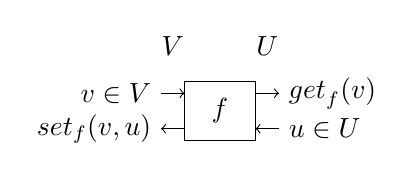
\begin{tikzpicture}[yscale=0.15,xscale=0.30,baseline=(V.base)]
    \draw (5,-1) rectangle (8,4) node[midway] {$f$};
    \draw[->] (4,3) node[left] (V) {$v \in V$} -- (5,3) node[above=1em,midway] (A2) {$V$};
    \draw[->] (8,3) -- (9,3) node[above=1em,midway] (A1) {$U$} node[right] {$\kw{get}_f(v)$};
    \draw[->] (9,0) node[right] {$u \in U$} -- (8,0);
    \draw[->] (5,0) -- (4,0) node[left] {$\kw{set}_f(v, u)$};
    \path (A1) -- node {$\rightleftarrows$} (A2);
  \end{tikzpicture}
\]
Operationally,
when an incoming question $v \in V$ activates the components,
the view $\kw{get}_f(v) \in U$ is extracted and
forwarded as an outgoing question.
When this outgoing question is answered with an update $u \in U$,
the updated value $\kw{set}_f(v, u)$ is returned to the caller.

\begin{definition}[Transition System from Lens]
  \label{ox:def:lts-lens}
  Given a lens $f : U \lensarrow V$,
  the transition system $\llbracket f \rrbracket : [U] \twoheadrightarrow [V]$
  is defined as
  \[
    \llbracket f \rrbracket \::=\:
    \langle
    V, =_V, =_V ,X_f, Y_f, =_V
    \rangle
    \qquad
    \begin{prooftree}
      \hypo{\kw{get}_f(v) = u}
      \infer1{v \mathbin{X_f} u}
    \end{prooftree}
    \qquad
    \begin{prooftree}
      \hypo{\kw{set}_f(v, u) = v'}
      \infer1{u \mathbin{Y_f}^v v'}
    \end{prooftree}
  \]
\end{definition}

As with $L \at U$,
$L \at f$ is written
when the lens $f$ is composed with an active component $L$:
\[
  L \at f \::=\: L \otimes \llbracket f \rrbracket \,.
\]

Similar to $L\at U$,
every question and answer consists of a pair:
one component from $A$ or $B$ handled by $L$,
and one component from the sets $U$ or $V$ carried along.
When $L$ makes an outgoing call,
the second component
is first passed through the lens $f$
to be projected into $U$:
\[
  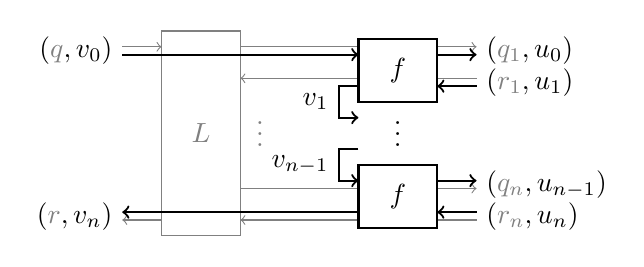
\begin{tikzpicture}[yscale=0.2,xscale=0.5]
    \begin{scope}[gray]%[canvas is xz plane at y=0,gray]
      \draw (-3,-2) rectangle (-1,11) node[midway] {$L$};
      %\scriptsize
      \draw[->] (-4,10) -- (-3,10);
      \draw[->] (-1,10) -- (5,10);
      \draw[->] (5,8) -- (-1,8);
      \draw[->] (-1,1) -- (5,1);
      \draw[->] (5,-1) -- (-1,-1);
      \draw[->] (-3,-1) -- (-4,-1);
      \node at (-0.5,5) {$\vdots$};
    \end{scope}
    \begin{scope}[thick,yshift=-0.5cm] %[canvas is xz plane at y=0.3]
      \draw[fill=white] (2,7) rectangle (4,11) node[midway] {$f$};
      \draw[fill=white] (2,-1) rectangle (4,3) node[midway] {$f$};
      \draw[->] (-4,10) -- (2,10);
      \draw[->] (4,10) -- (5,10);
      \draw[->] (5,8) -- (4,8);
      \draw[->] (4,2) -- (5,2);
      \draw[->] (5,0) -- (4,0);
      \draw[->] (2,0) -- (-4,0);
      \draw[->] (2,8) -- (1.5,8) -- node[left] {$v_1$} (1.5,6) -- (2,6);
      \draw[->] (2,4) -- (1.5,4) -- node[left] {$v_{n-1}$} (1.5,2) -- (2,2);
      \node at (3,5.5) {$\vdots$};
    \end{scope}
    \begin{scope}[yshift=-0.25cm]%[canvas is xz plane at y=0.15]
      \path
      (-4,10) node[left] {$(\textcolor{gray}{q}, v_0)$}
      ( 5,10) node[right] {$(\textcolor{gray}{q_1}, u_0)$}
      ( 5, 8) node[right] {$(\textcolor{gray}{r_1}, u_1)$}
      ( 5, 1.5) node[right] {$(\textcolor{gray}{q_n}, u_{n-1})$}
      ( 5,-0.5) node[right] {$(\textcolor{gray}{r_n}, u_n)$}
      (-4,-0.5) node[left] {$(\textcolor{gray}{r}, v_n)$};
    \end{scope}
  \end{tikzpicture}
\]

Lenses can be composed in a natural way.
\begin{definition}[Composition of Lenses]
  \label{ox:def:lens-comp}
  The identity lens $\kw{id}_U : U \lensarrow U$
  is given by
  \[
    \kw{get}_\kw{id}(u) = u
    \qquad
    \kw{set}_\kw{id}(u, u') = u'
  \]
  Given two lenses $f : U \lensarrow V$ and $g : V \lensarrow W$,
  the composition $g \circ f : U \lensarrow W$
  is given by
  \[
    \kw{get}_{g \circ f}(w) = \kw{get}_f(\kw{get}_g(w))
    \qquad
    \kw{set}_{g \circ f}(w, u') = \kw{set}_g(w, \kw{set}_f(\kw{get}_g(w), u'))
  \]
  The composition is associative,
  and the identity lens is the left and right identity of the composition.
  In other words,
  lenses form a category $\mathbf{Lens}$.
  In addition,
  the lenses are embedded functorially
  into the transition systems:
  \[
    \llbracket \kw{id}_U : U \lensarrow U \rrbracket \:\equiv\: \kw{id}_{U} : U \twoheadrightarrow U
    \qquad
    \llbracket g \circ f \rrbracket \:\equiv\: \llbracket g \rrbracket \odot \llbracket f \rrbracket
  \]
\end{definition}

In addition to its operational interpretation,
lenses can be viewed relationally,
as associating an original state with a transformed state.
This perspective allows
simulation conventions to be defined from a lens.
\begin{definition}[Simulation Conventions from Lens]
  \label{ox:def:sc-lens}
  Given a lens $f : U \lensarrow V$,
  \begin{itemize}
    \item
      the simulation convention $f^* : [U] \twoheadleftrightarrow [V]$
      is defined as
      \[
        f^* \::=\: \langle V, R_f^\que, R_f^\ans \rangle
        \qquad
        v \Vdash u \mathrel{R_f^\que} v \::\Leftrightarrow\: \kw{get}_f(v) = u
        \qquad
        v \Vdash u' \mathrel{R_f^\ans} v' \::\Leftrightarrow\: \kw{set}_f(v, u') = v'
      \]
    \item
      the simulation convention $f_* : [V] \twoheadleftrightarrow [U]$
      is defined by taking the inverse of $f^*$.
  \end{itemize}
\end{definition}

The simulation conventions $f^*$ and $f_*$
are compatible with the lens transition system
$\llbracket f \rrbracket$
in the sense that
the simulation squares
introduced in \autoref{def:ox:companion}
are satisfied.
\begin{theorem}
  Every lens-derived transition system
  $\llbracket f \rrbracket : [U] \twoheadrightarrow [V]$
  has a companion $f^* : [U] \twoheadleftrightarrow [V]$
  and a conjoint $f_* : [V] \twoheadleftrightarrow [U]$.
\end{theorem}

In practice,
two kinds of lens turn out to be especially useful.
First,
every bijection is a lens,
and this can be used to define structural isomorphisms
such as $\gamma_{U,V} : U \times V \cong V \times U$.
Secondly, the trivial lens
$\termi{V} : \mathbf{1} \leftrightarrows V$
where
$\kw{get}_{\termi{V}}(v) = *$ and
$\kw{set}_{\termi{V}}(v, *) = v$
can act as a ``terminator'',
which does not propagate any part of the state in $U$
but instead returns it unchanged to the caller.
The simulation convention
$\termi{U}^* : \mathbf{1} \twoheadleftrightarrow U$
introduced in \autoref{sec:ox:application}
is precisely the companion of this ``terminator'' lens,
which explains the chosen notation.

The properties of the generalized $\at$ operator
are summarized in Fig.~\ref{fig:xcomp}.

\begin{figure}
  \begin{gather*}
    \begin{prooftree}
      \hypo{L : A \twoheadrightarrow B}
      \hypo{f : U \lensarrow V}
      \infer2[\kw{ts}-$\at$]{
        L \at f : A \at U \twoheadrightarrow B \at V
      }
    \end{prooftree}
    \hspace{8em}
    \begin{prooftree}
      \hypo{\mathbf{R} : A \twoheadleftrightarrow B}
      \hypo{\mathbf{S} : U \twoheadleftrightarrow V}
      \infer2[\kw{sc}-$\at$]{
        \mathbf{R} \at \mathbf{S} : A \at U \twoheadleftrightarrow B \at V
      }
    \end{prooftree}
    \\[1em]
    \begin{array}{r@{}l}
      (L_1 \odot L_2) \at (f \circ g) & {} \equiv
      (L_1 \at f) \odot (L_2 \at g) \\
      \kw{id}_A \at \kw{id}_U & {} \equiv \kw{id}_{A \at U}
    \end{array}
    \quad
    \begin{array}{r@{}l}
      (\mathbf{R}_1 \vcomp \mathbf{R}_2) \at (\mathbf{S}_1 \vcomp \mathbf{S}_2)
      & {} \equiv
      (\mathbf{R}_1 \at \mathbf{S}_1) \vcomp (\mathbf{R}_2 \at \mathbf{S}_2)
      \\
      \idsc_A \at \idsc_U & {} \equiv \idsc_{A \at U}
    \end{array}
    \\[1em]
    \begin{prooftree}
      \hypo{\phi: L \le_{\mathbf{R}_1 \twoheadrightarrow \mathbf{S}_1} L'}
      \hypo{\psi: f \le_{\mathbf{R}_2 \twoheadrightarrow \mathbf{S}_2} f'}
      \infer2[\kw{sim}-$\at$]{\phi \at \psi :
        L \at f
        \le_{\mathbf{R}_1 \at \mathbf{R}_2 \twoheadrightarrow
        \mathbf{S}_1 \at \mathbf{S}_2}
      L' \at f'}
    \end{prooftree}
  \end{gather*}
  \caption{Spatial composition ($\mathbin@$) for strategies,
  simulation conventions and simulation proofs.}
  \label{fig:xcomp}
\end{figure}

\section{Summary}

This chapter develops OpenTX,
a three-dimensional algebraic compositional framework
that extends CompCertO with enhanced modularity capabilities.
The key contributions are threefold.
First, the layered composition operator $\odot$ enables horizontal composition
of components with heterogeneous interfaces,
addressing a fundamental limitation of CompCertO's linking operator.
Second, the state lifting operator $\at$ introduces spatial composition,
providing a flexible mechanism for managing abstract state
that was previously impossible in CompCertO.
Third, the extension of CompCert's memory model with a join operator
enables more modular reasoning about memory separation,
supporting composition patterns beyond those of the original framework.
Together, these enhancements create a semantic structure
where proof obligations decompose naturally along three orthogonal axes,
significantly improving the scalability of verification efforts.

The practical impact of these theoretical advances
is demonstrated through concrete case studies.
The bounded queue example illustrates how
complex correctness arguments that were previously monolithic
can be decomposed into independent, reusable components.
By aligning proof obligations with the three compositional axes,
the verification avoids entanglement between orthogonal concerns
and enables modular reasoning about the interaction
between high-level specifications and low-level implementations.
Similarly, the CAL framework instantiation shows how
layered systems can be verified incrementally,
with each layer proved in isolation
and correctness results combined systematically
through the algebraic structure.
This approach reduces verification complexity significantly.

Looking forward,
OpenTX provides a robust foundation for future work
in compositional verification.
The three-dimensional algebraic structure
not only preserves CompCertO's expressiveness and rigor
but fundamentally extends its reach
to verification scenarios that were previously intractable.
By enabling systematic decomposition of complex systems
into manageable, independently verifiable components,
OpenTX represents a significant step toward
making formal verification practical
for real-world systems of substantial complexity.
The next chapter builds upon this foundation
by exploring advanced techniques for state encapsulation,
further expanding the framework's applicability
to scenarios involving sophisticated abstract state management.
